% SCIENCE Visual Guide 2.0.1 + AI_SKILLS_R5; Akulin--Karlov batch v2.
% Graph traces are visibly heavier than axes. All labels use anchored positions.
\documentclass[border=5pt]{standalone}
\usepackage{fontspec,unicode-math}
\setmainfont{Noto Sans}
\setsansfont{Noto Sans}
\setmathfont{STIXTwoMath-Regular.otf}
\usepackage{tikz}
\usetikzlibrary{arrows.meta,calc,patterns,decorations.pathreplacing,intersections}
\definecolor{ScienceInk}{HTML}{000000}
\definecolor{ScienceCurve}{HTML}{000000}
\definecolor{ScienceAux}{HTML}{000000}
\definecolor{ScienceMuted}{HTML}{000000}
\tikzset{
  axis/.style={draw=ScienceInk,line width=0.75pt,-{Latex[length=2.2mm,width=1.35mm]}},
  axisplain/.style={draw=ScienceInk,line width=0.70pt},
  curve/.style={draw=ScienceCurve,line width=2.15pt,line cap=round,line join=round},
  curveb/.style={draw=ScienceAux,line width=1.95pt,dash pattern=on 6pt off 2.4pt,line cap=round,line join=round},
  curvedash/.style={draw=ScienceAux,line width=1.9pt,dash pattern=on 4pt off 3pt},
  optbeam/.style={draw=ScienceCurve,line width=1.75pt,-{Latex[length=2.2mm,width=1.3mm]}},
  optback/.style={draw=ScienceAux,line width=1.65pt,-{Latex[length=2mm,width=1.2mm]}},
  opt/.style={draw=ScienceInk,line width=1.0pt},
  opticplate/.style={draw=ScienceInk,line width=1.02pt,pattern=north east lines,pattern color=ScienceMuted},
  tick/.style={draw=ScienceInk,line width=0.7pt},
  textlabel/.style={text=ScienceInk,font=\fontsize{15}{18}\selectfont},
  smalllabel/.style={text=ScienceInk,font=\fontsize{13.5}{16.2}\selectfont},
}
\begin{document}
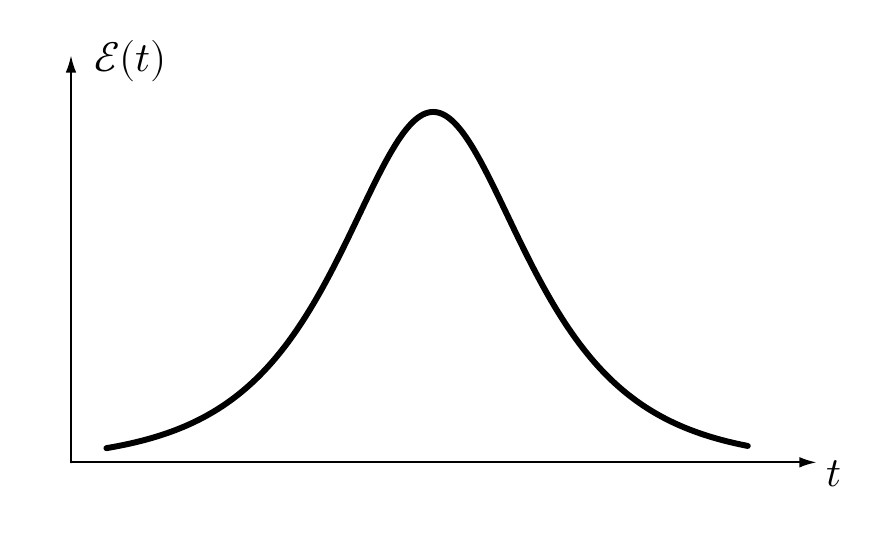
\begin{tikzpicture}[x=1cm,y=1cm,>=Latex,line cap=round,line join=round,font=\fontsize{15}{18}\selectfont]


% 2π SIT: sech envelope; axis title anchored at arrow height.
\path[use as bounding box] (0,0) rectangle (10.45,6.2);
\draw[axis] (.55,.68)--(10.02,.68);
\draw[axis] (.55,.68)--(.55,5.85);
\node[textlabel,anchor=west] at (.72,5.78) {$\mathscr E(t)$};
\node[textlabel,anchor=west] at (10.02,.54) {$t$};
\draw[curve,samples=360,domain=1:9.15,smooth] plot (\x,{.68+4.45/(cosh(0.94*(\x-5.15)))});

\end{tikzpicture}
\end{document}
